\section{Data Overview}
In this analysis, I employ an unsupervised machine learning approach to address fundamental questions in labour economics. I begin by outlining the methodology and data preparation techniques used prior to the algorithmic modeling. My primary data source is the Understanding Society: UK Household Longitudinal Study (UKHLS), a comprehensive longitudinal panel study spanning 13 years. This study serves as a continuation of the British Household Panel Study (BHPS), which ran from 1991 to 2008.

I extracted relevant health variables in a long panel format, focusing on two key aspects of health deficits: chronic illnesses and substantial difficulties caused by health problems or disabilities \citep{ukhls_disdif6}. Chronic illnesses in the survey include diagnosed conditions such as asthma, arthritis, cancer, and high blood pressure. While my analysis follows \citet{denardi2024wp}, I place greater emphasis on chronic illnesses \citep{borella_nber}. The difficulties/disability variables, in contrast, are not necessarily diagnoses but rather descriptions of challenges in daily activities, such as ``difficulty with moving objects'' or ``difficulty with daily tasks.''

The focus on chronic illness is crucial due to its pervasive impact on individuals and healthcare systems. The National Institutes of Health (NIH) defines chronic conditions as persistent health issues lasting more than three months, encompassing a range of ailments including arthritis, asthma, cancer, diabetes, and certain viral diseases \citep{bernell2016}. The World Health Organization categorizes these as non-communicable diseases, characterized by their long-lasting nature and slow progression, primarily including cardiovascular diseases, cancers, chronic respiratory diseases, and diabetes \citep{who_ncd}. By examining chronic illnesses, this paper address a significant aspect of public health that has profound implications for labour market participation and economic outcomes. The enduring nature of these conditions necessitates a deeper understanding of how they shape individuals' health trajectories and, consequently, their long-term economic prospects.

In the UKHLS dataset, health deficits are recorded as 1 (present/diagnosed), 0 (not present), or -9 (refusal/not applicable). For my analysis, I converted any value other than 1 or 0 to Python's undefined data format --- \texttt{NaN}. To account for the nuanced recording methods in the UKHLS survey, I created a new ``healthcond'' variable that aggregates all variations of the ``hcond'' variables. This new variable operates under the assumption that once a person is diagnosed with a chronic illness, such as asthma, they continue to have it until the end of the survey or their death. In total, my analysis incorporates 16 variables related to chronic illnesses and 11 difficulty/disability variables across 13 waves of data.

These 27 variables are used to construct the key variable of interest --- ``frailty.'' The frailty variable provides a snapshot of an individual's health at a given point in time. It is calculated by dividing the number of an individual's health deficits by the total number of possible health deficits. This approach yields a normalized measure ranging from 0 to 1, where 0 represents perfect health (no deficits) and 1 represents the most extreme poor health (all deficits present or death).

For instance, an individual with no health deficits will have a frailty score of 0, while an individual who dies will have a frailty score of 1 in the corresponding wave, as death represents the ultimate manifestation of poor health. It's important to note that death data is available only for existing participants, totaling 4,444 individuals across the UKHLS survey lifespan. The wave data continues to be recorded even after an individual's death, maintaining the continuity of the dataset.

The calculation of the frailty variable involves a nuanced approach to handling missing data:
\begin{enumerate}
    \item If all health conditions are recorded as \texttt{NaN} across all waves for an individual, the frailty is set to \texttt{NaN} for all waves of that person.
    \item For individuals with at least some health data, frailty is calculated for each wave, treating \texttt{NaN} values as 0 in the calculation. This approach assumes that missing data indicates the absence of a health deficit, which may introduce a slight bias towards lower frailty scores in cases of incomplete data.
    \item If an individual has no health data across all waves, their frailty is set to \texttt{NaN} for all waves, effectively excluding them from analyses that require this variable.
\end{enumerate}

The summary statistic and distribution of the frailty data are shown in Figure~\ref{fig:frailty_dist}, and the binned relationship between age and frailty is shown in Figure~\ref{fig:frailty_age}.

\begin{figure}[ht]
    \centering
    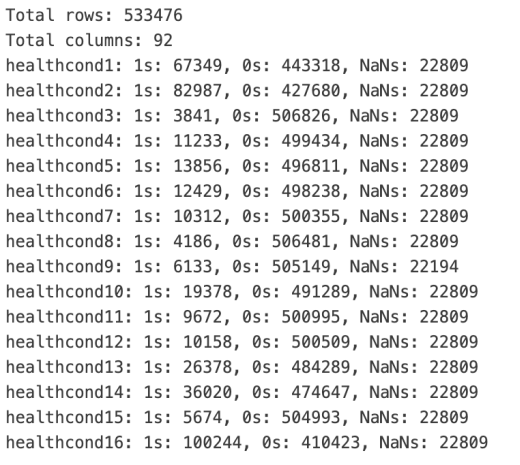
\includegraphics[width=0.85\textwidth]{figures/fig-000.png}
    \caption{Summary distribution of frailty (extracted from the original dissertation PDF).}
    \label{fig:frailty_dist}
\end{figure}

\begin{figure}[ht]
    \centering
    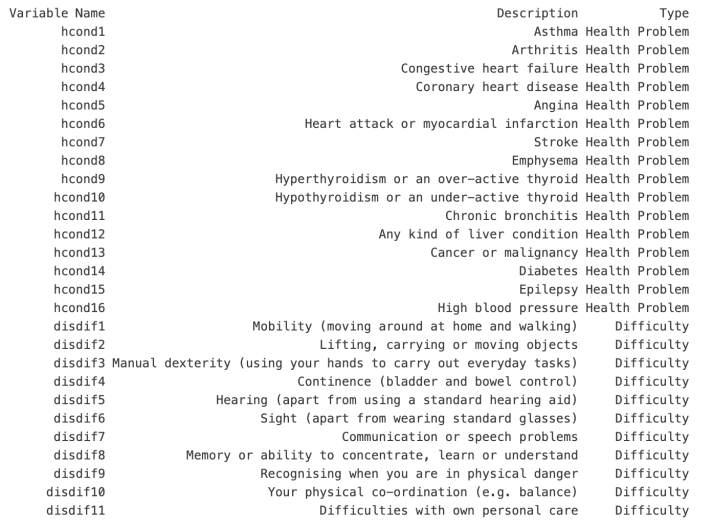
\includegraphics[width=0.85\textwidth]{figures/fig-001.png}
    \caption{Binned relationship between age and frailty (extracted from the original dissertation PDF).}
    \label{fig:frailty_age}
\end{figure}

The survey assigns a frailty score of 1 to all individuals above 105 years old. This decision is based on two factors:
\begin{enumerate}
    \item The extreme rarity of survival beyond this age.
    \item Research indicating that the risk of mortality plateaus after age 105, rather than continuing to increase exponentially as it does from age 60 onwards.
\end{enumerate}
This approach ensures that the frailty measure accounts for the unique health characteristics of extreme longevity while maintaining consistency in the data analysis. It also aligns with current understanding of mortality patterns in very advanced age groups \citep{nlm_age105}.

The data reveals a clear upward trajectory in frailty after age 60, which can be attributed to dramatic age-related changes in the human immune system. This observation aligns with recent findings published in \textit{Nature Aging} \citep{shen2024}, which document significant alterations in immune cell populations and functions with advancing age. These findings provide a potential explanation for the upward trend in health issues post-60 observed in the data, linking biological mechanisms to population-level health trajectories.
